\documentclass[aspectratio=169]{beamer}  % 16:9 宽屏
\usefonttheme[onlymath]{serif} % 保留数学公式的手写体风格
\usepackage[UTF8]{ctex}                  % 中文支持
\usepackage{fontspec}                    % 字体设置
\usepackage{graphicx}                    % 插图支持
\usepackage{amsmath,amssymb,amsfonts,amsthm}            % 数学公式支持
\usepackage{tikz}                        % 绘图支持
\usepackage{hyperref} % 超链接支持

\usepackage{listings}
\usepackage{xcolor} % 颜色支持

% 代码配色(算法竞赛常用风格)
% \lstdefinestyle{codeblockstyle}{
%     basicstyle=\ttfamily\small,
%     keywordstyle=\color{blue}\bfseries,
%     commentstyle=\color{green!50!black},
%     stringstyle=\color{orange},
%     numbers=left,
%     numberstyle=\tiny,
%     breaklines=true
% }

\hypersetup{
    % colorlinks=true,
    % linkcolor=blue,
    % urlcolor=blue,
    % pdfborder={0 0 1} % 链接边框: 0 0 1 表示下划线
}

\lstset{
    language=C++,
    basicstyle=\ttfamily\small,
    keywordstyle=\color{blue}\bfseries,
    commentstyle=\color{green!50!black},
    stringstyle=\color{orange},
    numbers=left,
    numberstyle=\tiny,
    numbersep=6pt, % 行号和代码的间距
    xleftmargin=2em, % 让行号+代码整体右移
    % frame=single, % 给代码加外框
    breaklines=true
}

% 自定义代码块环境
\newenvironment{codeblock}[1][代码]{
    \setbeamercolor{block title}{fg=white,bg=black!80!blue}
    \setbeamercolor{block body}{bg=black!5!white,fg=black}
    \begin{block}{#1}
}{
    \end{block}
}

\newcounter{quizcounter}

\newenvironment{quizblock}{
    \refstepcounter{quizcounter}% 计数器加1
    \setbeamercolor{block title}{fg=white,bg=orange!85!black} % 标题背景
    \setbeamercolor{block body}{bg=orange!10!white,fg=black}   % 内容背景
    \begin{block}{Quiz \arabic{quizcounter}}
}{
    \end{block}
}

% 字体设置(可按需替换)
\setmainfont{Times New Roman}
\setsansfont{Arial}

% Beamer 主题(可改为其他主题如 Madrid、Frankfurt 等)
% \usetheme{Berlin}
\usetheme{Frankfurt}
% \usecolortheme{beetle	}

% 页脚设置
\setbeamertemplate{footline}[frame number]

\newcommand{\R}{\mathbb{R}}
\newcommand{\N}{\mathbb{N}}
\newcommand{\Z}{\mathbb{Z}}
\newcommand{\pau}{\pause}

% 封面信息
\title{数学基础}
\subtitle{2025 暑期留校集训}
\author{$\mathbf{99\_wood}$}
\institute{东北大学\\计算机科学与工程学院}
\date{\today}
\logo{
\includegraphics[width=1cm]{./figure/logo.png}}

\begin{document}

% 封面页
\begin{frame}
  \titlepage
\end{frame}

\begin{frame}{开始之前}
  \pau
  \begin{itemize}
    \item 算法竞赛 $\neq$ 数学竞赛. \pau
    \item 但是随着你不断深入算法竞赛, 数学知识会变得越来越重要. 没有良好的数学素养, 很难在算法竞赛中取得好成绩. \pau
    \item 虽然在比赛当中你可以猜猜猜, 但是在你学习数学知识时,
          还是要怀着严谨的心态. 多思考, 多感悟.
  \end{itemize}
  \begin{figure}
    \centering
    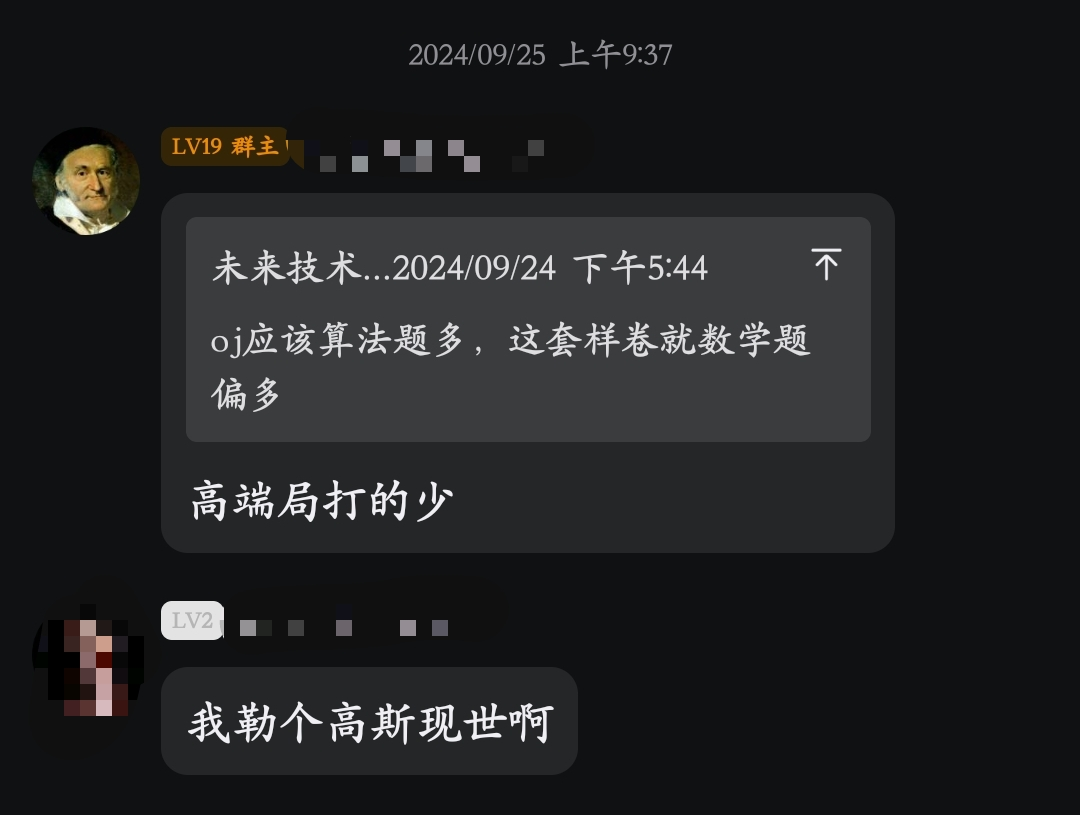
\includegraphics[width=0.3\textwidth]{./figure/gaoduanjv.jpg}
    % \caption{数学的美}
  \end{figure}
\end{frame}

% 目录页
\begin{frame}{目录}
  \tableofcontents
\end{frame}

\section{数学思想}

% --- 数学思维总览 ---
\begin{frame}{数学思想总览}
在算法竞赛中, 数学知识不仅仅是公式和定理, 更重要的是\alert{思想与方法}.
常见的数学型思路包括: 
\begin{columns}[t]
    \column{0.5\textwidth}
    \begin{enumerate}
        \item 拆项与化简
        \item 交换枚举顺序
        \item 算贡献
        \item 容斥原理
        \item 转化思想
    \end{enumerate}

    \column{0.5\textwidth}
    \begin{enumerate}
        \setcounter{enumi}{5}
        \item 分块思想
        \item 分类讨论
        \item 利用单调性
        \item 前缀和与差分
        \item 二进制分解
    \end{enumerate}
\end{columns}

\vspace{1em}

这些是构建数学解题思维的常用工具箱. 
\end{frame}

% --- 拆项与化简 ---
\begin{frame}{拆项与化简}
\begin{block}{核心思想}
将复杂的表达式拆解为简单的可处理部分, 通过代数变形化简计算量. 
\end{block}
\pau
\begin{example}
求和式 $\displaystyle \sum_{k=1}^n k(k+1)$. \pau
\[
\sum_{k=1}^n k^2 + k
= \left(\sum_{k=1}^n k^2\right) + \left(\sum_{k=1}^n k\right)
= \frac{n(n+1)(2n+1)}{6} + \frac{n(n+1)}{2}
\]
利用公式直接求得结果, 避免逐项计算.
\end{example}
\end{frame}

% --- 交换枚举顺序 ---
\begin{frame}{交换枚举顺序}
\begin{block}{核心思想}
在双重或多重循环(或求和)中, 改变枚举顺序, 让复杂问题转化为易计算的形式. 
\end{block}
\pau

\begin{example}
统计所有 $(i,j)$ 满足 $1 \le j \le i \le n$
$$\sum_{i=1}^n \sum_{j=1}^i \lfloor \frac{i}{j} \rfloor$$
\end{example}
\end{frame}

\begin{frame}{交换枚举顺序}
\begin{solution}
令 $l = \lfloor \frac{n - j + 1}{j} \rfloor = \lfloor \frac{n + 1}{j} \rfloor - 1$
\begin{align*}
\sum_{i=1}^n \sum_{j=1}^i \lfloor \frac{i}{j} \rfloor
&= \sum_{j=1}^n \sum_{i=j}^n \lfloor \frac{i}{j} \rfloor\\
&= \sum_{j=1}^n \left(\sum_{k=1}^{l} kj + (n - (l + 1)j + 1)(l + 1)\right)\\
&= \sum_{j=1}^n \left(j \sum_{k=1}^{l} k + (n - (l + 1)j + 1)(l + 1)\right)\\
&= \sum_{j=1}^n \left(j \frac{l(l + 1)}{2} + (n - (l + 1)j + 1)(l + 1)\right)\\
\end{align*}
\end{solution}
\end{frame}

\begin{frame}{交换枚举顺序}
\begin{solution}
\begin{align*}
\sum_{i=1}^n \sum_{j=1}^i \lfloor \frac{i}{j} \rfloor
&= \sum_{j=1}^n \left(j \frac{l(l + 1)}{2} + (n - (l + 1)j + 1)(l + 1)\right)\\
&= \sum_{j=1}^n j \frac{l(l + 1)}{2} + \sum_{j=1}^n(n - (l + 1)j + 1)(l + 1) \\
\end{align*}
这里就可以在 $O(n)$ 的时间复杂度内计算出结果.

\vspace{1em}

如果你会数论分块, 还可以在 $O(\sqrt{n})$ 的时间复杂度内计算出结果.
\end{solution}
\end{frame}

% --- 贡献法 ---
\begin{frame}{算贡献}
\begin{block}{核心思想}
不直接遍历所有组合, 而是固定一个元素, 计算它对整体答案的贡献. 
\end{block}
\pau

\begin{example}
求数组所有子段的和. 
\pau

\vspace{1em}

固定 $a_k$, 它出现在多少个子段里?
左边可选 $k$ 种起点, 右边可选 $n-k+1$ 种终点, 总贡献: 
\[
a_k \times k \times (n-k+1)
\]
总和为 $\displaystyle \sum_{k=1}^n a_k \cdot k \cdot (n-k+1)$. 
\end{example}
\end{frame}


\begin{frame}[fragile]{快速幂}
\begin{block}{思路}
利用二进制拆分指数, 将幂运算的时间复杂度从 $O(n)$ 降为 $O(\log n)$: 
\[
a^b =
\begin{cases}
(a^{b/2})^2, & b \ \text{为偶数}\\
a \times (a^{b-1}), & b \ \text{为奇数}
\end{cases}
\]
\end{block}

\begin{example}
计算 $3^{13}$: 
\[
3^{13} = 3 \times (3^6)^2
= 3 \times (3^3)^4
= 3 \times (3 \times 3^2)^4
\]
\end{example}
\end{frame}


\begin{frame}[fragile]{快速幂}
\begin{codeblock}
\begin{lstlisting}[language=C++]
int qpow(int a, int b, int mod) {
    int res = 1;
    while (b) {
        if (b & 1) res = 1ll * res * a % mod;
        a = 1ll * a * a % mod;
        b >>= 1;
    }
    return res;
}
\end{lstlisting}
\end{codeblock}
\end{frame}


\section{整除}
\begin{frame}{整除}
    \begin{definition}
      对于 $d, a \in \mathbb{Z}, d \neq 0$, 如果存在 $k \in \mathbb{Z}$, 使得 $a = k \cdot d$, 则称 $d \mid a$ ($d$ 整除 $a$).
    \end{definition}
  \begin{itemize}
    \item $\mid$ 是整除符号.
    \item $d$ 是 $a$ 的约数, $a$ 是 $d$ 的倍数.
  \end{itemize}
\end{frame}

\begin{frame}{性质}
  整除关系有以下性质:
  \pau

  \vspace{1em}

  \begin{itemize}
    \item 自反性: 对于任意整数 $n \neq 0$, 有 $n \mid n$.\pau
    \item 反对称性: 若有 $a \mid b$ 且 $|a| \neq |b|$, 则 $b \nmid a$.\pau
    \item 传递性: 若有 $a \mid b, b \mid c$, 则 $a \mid c$.\pau
    \item $\forall a \in \mathbb{Z} \land a \neq 0, a \mid 0$.\pau
    \item $\forall a \in \mathbb{Z}, 1 \mid a$.\pau
    \item $a \mid b, a \mid c \Leftrightarrow
          \forall x, y \in \mathbb{Z}, a \mid (bx + cy)$.\pau
    \item $m \neq 0, a \mid b \Leftrightarrow
          ma \mid mb$.\pau
  \end{itemize}
  
  \vspace{1em}

  这说明自然数集上的整除关系是一个偏序关系.
\end{frame}

\begin{frame}{约数}
  \begin{definition}
  如果 $a \mid b$, 那么 $a$ 是 $b$ 的约数, $b$ 是 $a$ 的倍数.
  也称 $a$ 为 $b$ 的因子.
  \end{definition}


  \begin{corollary}
  任何数 $n$ 至少有两个因子: $1$ 和 $n$ 自身.
  我们将它们称为 $n$ 的平凡因子.
  \end{corollary}
  
\end{frame}

\begin{frame}{Quiz}
  \begin{quizblock}
    $[1,n]$ 的整数中, $k$ 的倍数有多少个?
  \end{quizblock}\pau

  \begin{solution}
    $[1,n]$ 中 $k$ 的倍数一次为 $k, 2k, \ldots, mk$.
    其中 $m = \lfloor \frac{n}{k} \rfloor$.
    因此答案为 $\lfloor \frac{n}{k} \rfloor$.
  \end{solution}
\end{frame}


\begin{frame}{Quiz}
  \begin{quizblock}
    如何计算 $[1,n]$ 中每个数的约数个数 $d(n)$?
    要求复杂度为 $\mathcal{O}(n\log{n})$ 级别.
  \end{quizblock}\pau
  \begin{solution}
    我们可以使用筛法来计算 $[1,n]$ 中每个数的约数个数 $d(n)$.

    具体步骤如下:
    \begin{itemize}
      \item 初始化一个大小为 $n+1$ 的数组 $d$, 全部赋值为 $0$.
      \item 对于每个整数 $i \in [1,n]$, 将 $i$ 的所有倍数 $j$ 的约数个数 $d(j)$ 加 $1$.
    \end{itemize}

    这个复杂度为 $\displaystyle \sum_{i=1}^{n} \frac{n}{i} = n \sum_{i=1}^{n} \frac{1}{i} = \mathcal{O}(n\ln{n})$ 的.
    (注意这个调和级数的求和技巧经常用到)

    这样我们就可以在 $\mathcal{O}(n\ln{n})$ 的时间复杂度内计算出每个数的约数个数.
  \end{solution}
\end{frame}

\section{质数}

\begin{frame}{质数}
  \begin{definition}
    大于 $1$ 的自然数中, 只有 $1$ 和它本身两个因子的数叫做质数.

    反之, 如果一个数有超过两个因子, 则称它为合数.

    \textbf{$1$ 既不是质数也不是合数.}
  \end{definition}
  \begin{example}
    $2, 3, 5, 7, 11, 13, 17, 19, 23, 29, 31, 37, 41, 43, 47, \ldots$ 等都是质数.
  \end{example}
\end{frame}

\begin{frame}{Quiz}
  \begin{quizblock}
    质数有无数个. 如何证明?

  \end{quizblock}\pau
  \begin{proof}
    考虑反证法: 

    假设质数是有限的, 则可以列出所有质数 $p_1, p_2, \ldots, p_n$.

    考虑数 $N = p_1 p_2 \cdots p_n + 1$.

    显然 $N$ 不是任何 $p_i$ 的倍数, 因此 $N$ 是质数.
    这与假设矛盾, 所以质数有无数个.
  \end{proof}
\end{frame}

\begin{frame}{质数的分布}
虽然我们目前没有摸清楚质数的具体分布情况, 但是我们能给出近似的: 

\vspace{1em}

设 $\pi(n)$ 为不超过 $n$ 的质数个数. 那么有: 

$$\pi(n) \sim \frac{n}{\ln n}$$

\end{frame}

\begin{frame}[fragile]{判断质数}

  我们可以在 $\mathcal{O}(\sqrt{n})$ 的时间复杂度内判断 $n$ 是不是质数.

  \vspace{1em}

  \begin{codeblock}
    \begin{lstlisting}[language=C++]
bool isPrime(const int x) {
    if(x == 1) return false;
    for(int i = 2; i * i <= x; ++i){
        if(x % i == 0) return false;
    }
    return true;
}
    \end{lstlisting}
  \end{codeblock}
  
\end{frame}

\begin{frame}{找质数}
  
  \begin{problem}
    如何求出 $[1,n]$ 中的所有质数?
  \end{problem}\pau

  \vspace{1em}
  
  朴素想法是逐个判断, 然而很不幸它的复杂度是

  $$\sum_{i=1}^{n} \sqrt{i} = O(n\sqrt{n})$$.

\end{frame}

\begin{frame}{埃氏筛}
  \pau
  我们可以采用前面提到的筛法.\pau
  
  \vspace{1em}
  
  筛法是一种高效的找出质数的方法, 最著名的就是\textbf{埃拉托斯特尼筛法}.\pau
  
  \vspace{1em}

  首先, 我们筛掉 $2$ 的倍数, 然后筛掉 $3$ 的倍数, 然后筛掉 $5$ 的倍数\dots\pau

  \vspace{1em}

  剩下来的数就是质数.

\end{frame}

\begin{frame}[fragile]{埃氏筛}
  \begin{codeblock}
    \begin{lstlisting}[language=C++]
bool isPrime[MAXN];
std::vector<int> prime;
void sieve(const int n) {
    for(int i = 1; i <= n; ++i) isPrime[i] = true;
    isPrime[1] = false;
    for(int i = 2; i <= n; ++i){
        if(isPrime[i]){
            prime.push_back(i);
            for(int j = i; 1ll * j * i <= n; ++j){
                isPrime[j * i] = false;
            }
        }
    }
}
    \end{lstlisting}
  \end{codeblock}
\end{frame}

\begin{frame}[fragile]{埃氏筛}

  埃氏筛的复杂度是 $\mathcal{O}(n\log\log n)$.\pau
  
  \vspace{1em}

  一个不太严谨的证明是我们之前提到的根据质数的分布规律,

  $$T = \sum_{p \text{ 是质数}} \frac{n}{p} \sim \ln\ln n \text{.}$$\pau
  
  因此, 埃氏筛的总时间复杂度为

  $$\mathcal{O}(n \ln\ln n) \text{.}$$\pau
  
  严谨的证明可以参考 \href{https://oi-wiki.org/math/number-theory/sieve/}{\color{magenta}\underline{OI-wiki}}.
\end{frame}

\begin{frame}{欧拉筛}

  但是我们注意到, 一些数会被多次筛去. 比如 $2 \mid 6$ 并且 $3 \mid 6$, 所以 $6$ 会被 $2$ 和 $3$ 两次筛去.\pau
  
  \vspace{1em}

  为了避免这种情况, 我们可以在筛选时只考虑每个质数的最小倍数. 这就是\textbf{欧拉筛}.\pau
  
  \vspace{1em}

  显然每个数只会被它的最小质因子筛去一次. 这样, 我们就可以在 $\mathcal{O}(n)$ 的时间复杂度内找出所有质数.
\end{frame}

\begin{frame}[fragile]{欧拉筛}
  \begin{codeblock}
    \begin{lstlisting}[language=C++]
std::vector<int> prime;
int d[MAXN];
void sieve(int n) {
    for(int i = 2; i <= n; ++i){
        if(d[i] == 0){
            prime.push_back(i);
            d[i] = i;
        }
        for(const int p : prime){
            if(p > d[i] || 1ll * p * i > n) break;
            d[p * i] = p;
        }
    }
}
    \end{lstlisting}
  \end{codeblock}
\end{frame}

\begin{frame}{唯一分解定理}

  每个数都可以拆成质数乘积的方式. 这个过程叫做质因数分解.
  \pau
  \begin{example}
    \vspace{-1em}
    \begin{align*}
      5 &= 5 = 5^1\\
      15 &= 3 \times 5 = 3^1 \times 5^1\\
      36 &= 2 \times 2 \times 3 \times 3 = 2^2 \times 3^2\\
    \end{align*}
    \vspace{-3em}
  \end{example}\pau

  这样的分解方式是唯一的! 这就是\textbf{唯一分解定理}, 也叫\textbf{算术基本定理}.\pau

  \vspace{1em}

  分解某个数的质因数可以通过枚举所有小于等于 $\sqrt{n}$ 的数来实现, 复杂度为 $\mathcal{O}(\sqrt{n})$.
\end{frame}

\begin{frame}{Quiz}
  \begin{quizblock}
    如果我们把 $A$ 分解成了 $2^{a_1} 3^{a_2} 5^{a_3} \cdots$,
    把 $B$ 分解成了 $2^{b_1} 3^{b_2} 5^{b_3} \cdots$.

    那么 $A \times B$ 如何表示? 如何判断 $A \mid B$ 是否成立?
  \end{quizblock}\pau

  \begin{solution}
    \begin{itemize}
      \item $A \times B = 2^{a_1 + b_1} 3^{a_2 + b_2} 5^{a_3 + b_3} \cdots$
      \item $A \mid B$ 当且仅当 $\forall i, a_i \leq b_i$.
    \end{itemize}
  \end{solution}
\end{frame}

\begin{frame}{Quiz}
  \begin{quizblock}
    应用Quiz 4的结论. 给定 $n$ 的质因数分解形式 $2^{a_1} 3^{a_2} 5^{a_3} \cdots$ 如何快速求出 $d(n)$?
  \end{quizblock}\pau

  \begin{solution}
    根据质因数分解的性质, 我们有

    $$d(n) = (a_1 + 1)(a_2 + 1)(a_3 + 1) \cdots$$

    因此, 我们只需要在分解时记录每个质因子的指数即可.
  \end{solution}
\end{frame}

\section{公因数与公倍数}

\begin{frame}{公因数与公倍数}
  \begin{definition}
    对于两个整数 $a, b$, 如果存在一个整数 $d$ 使得 $d \mid a$ 且 $d \mid b$, 则称 $d$ 是 $a$ 和 $b$ 的公因数.
    最大的公因数称为 $\gcd(a, b)$, 也记为 $(a, b)$.
  \end{definition}

  \begin{definition}
    对于两个整数 $a, b$, 如果存在一个整数 $m$ 使得 $a \mid m$ 且 $b \mid m$, 则称 $m$ 是 $a$ 和 $b$ 的公倍数.
    最小的公倍数称为 $\operatorname{lcm}(a, b)$, 也记为 $[a, b]$.
  \end{definition}
\end{frame}
\begin{frame}{Quiz}
  \begin{quizblock}
    如果我们把 $A$ 分解成了 $\displaystyle \prod p_i^{a_i}$,
    把 $B$ 分解成了 $\displaystyle \prod p_i^{b_i}$.

    $\gcd(A,B)$ 和 $\operatorname{lcm}(A,B)$ 的表达式是什么?
  \end{quizblock}\pau

  \begin{solution}
    $$\gcd(A, B) = \prod p_i^{\min(a_i, b_i)}$$
    $$\operatorname{lcm}(A, B) = \prod p_i^{\max(a_i, b_i)}$$
  \end{solution}
\end{frame}

\begin{frame}{最大公因数与最小公倍数的性质}
  
  最大公因数与最小公倍数有以下性质:\pau

  \vspace{1em}

  \begin{itemize}
    \item $\forall d, d \mid a \land d \mid b \Leftrightarrow d \mid \gcd(a, b)$.\pau
    \item $\forall m, a \mid m \land b \mid m \Leftrightarrow \operatorname{lcm}(a, b) \mid m$.\pau
    \item $\gcd(a, b) \times \operatorname{lcm}(a, b) = a \times b$.\pau
    \item $\gcd(a, 0) = |a|$, $\operatorname{lcm}(a, 0) = 0$.\pau
    \item $\gcd(a, 1) = 1$, $\operatorname{lcm}(a, 1) = |a|$.\pau
    \item $\gcd(ka, kb) = k\gcd(a, b)$.\pau
    \item $\operatorname{lcm}(ka, kb) = k\operatorname{lcm}(a, b)$.\pau
    \item $\gcd(a, b) = \gcd(a, a \pm b)$.\pau
    \item $\gcd(a, b) = \gcd(b, a \bmod b) \quad (b \neq 0)$.
  \end{itemize}
\end{frame}

\begin{frame}{欧几里得算法}
  \begin{quizblock}
    如何证明 $\gcd(a, b) = \gcd(b, a \bmod b) \quad (b \neq 0)$.
  \end{quizblock}\pau
  
  \begin{solution}
    \begin{figure}
      \centering
      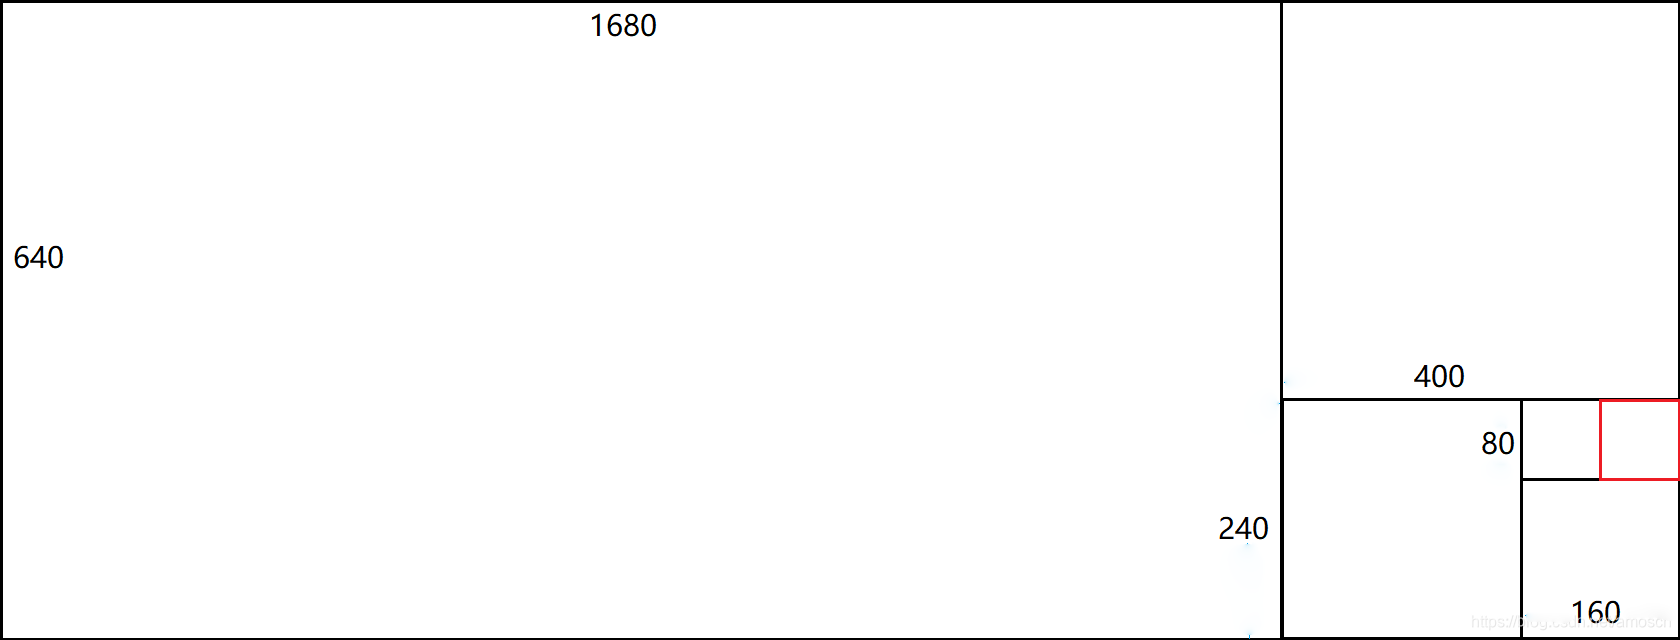
\includegraphics[width=0.8\textwidth]{./figure/proof1.png}
    \end{figure}
  \end{solution}

\end{frame}

\begin{frame}[fragile]{欧几里得算法}
  我们可以根据以上性质来快速求出 $\gcd(a, b)$.
  \begin{codeblock}
    \begin{lstlisting}[language=C++]
int gcd(int x, int y) {
    return y == 0 ? x : gcd(y, x % y);
}
    \end{lstlisting}
  \end{codeblock}

\end{frame}

\begin{frame}[fragile]{欧几里得算法}

  对于最小公倍数, 我们可以根据性质 $\gcd(a, b) \times \operatorname{lcm}(a, b) = a \times b$ 来求解.

  \begin{codeblock}
    \begin{lstlisting}[language=C++]
int lcm(int x, int y) {
    return x / gcd(x, y) * y;
}
    \end{lstlisting}
  \end{codeblock}\pau

  实际上, 对于 C++17, 我们可以使用 <numeric> 头文件中的 std::gcd 与 std::lcm 来求最大公约数和最小公倍数.
\end{frame}

\section{模意义下运算及扩展欧几里得算法}

\begin{frame}{取模}

  虽然我们对于取模已经习以为常, 但是我们还是有必要明确它的定义.\pau

  \vspace{1em}

  普遍地, 我们可以这样表达除法: 

  $$a = \lfloor \frac{a}{p} \rfloor \times p + a \bmod p$$

  其中 $p$ 是除数, $\lfloor \frac{a}{p} \rfloor$ 是商, $a \bmod p$ 是余数.

  \vspace{1em}
  
  这里的 $a \bmod p$ 就是我们常说的取模运算.
\end{frame}

\begin{frame}{模运算的性质}  
  值域: 由于模是取余, 所以 $a \bmod p$ 一定落在 $[0,p-1]$ 之间.\pau

  \vspace{1em}

  随时取模性质: 在\textbf{只含加法和乘法}的式子中, 如果最后的运算结果需要对 $p$ 取模, 那么我们可以在运算过程中随便取模.
  只需要最后把结果对 $p$ 再取模, 答案就是正确的.\pau

  \vspace{1em}

  由于这两条好用的性质, 所以很多题目都会要求我们输出模意义的结果, 以此避免精度问题.
  常用的模数有 $10^9 + 7$ 和 $998244353$. 这两个数都是质数.\pau
\end{frame}

\begin{frame}{乘法逆元}
  我们前面提到随时取模原理适用于\textbf{只含加法和乘法}的式子.
  但是很多时候我们需要用到除法, 那么除法是否适用随时取模原理呢?\pau
  
  \vspace{1em}

  答案是否定的. 因为即便取模后, 我们也无法保证模完的数能够整除分子.\pau

  \vspace{1em}

  能否找到一种方法来表示模意义下的分数呢?\pau

  \vspace{1em}

  这里我们引入乘法逆元的概念. 
  
  \begin{definition}
    在模 $p$ 意义下, 如果存在一个整数 $b$ 使得
    $$a \times b \equiv 1 \pmod{p} \text{.}$$
    这个 $b$ 就是 $a$ 的乘法逆元, 记作 $a^{-1}$.
  \end{definition}
\end{frame}

\begin{frame}{乘法逆元}
  \begin{definition}
    在模 $p$ 意义下, 如果存在一个整数 $b$ 使得
    $$a \times b \equiv 1 \pmod{p} \text{.}$$
    这个 $b$ 就是 $a$ 的乘法逆元, 记作 $a^{-1}$.
  \end{definition}\pau

  \vspace{1em}

  我们发现, 这里的 $b$ 具有类似于 $\dfrac{1}{a}$ 的功能. 
  当我们需要计算 $\displaystyle \dfrac{c}{a} \pmod{p}$ 时, 可以将其转化为 $c \times b \pmod{p}$.
\end{frame}

\begin{frame}{求逆元}
  求逆元主要有以下几种方法:\pau
  \begin{itemize}
    \item 费马小定理: 当 $p$ 是质数时, 有 $a^{p-1} \equiv 1 \pmod{p}$, 因此 $a^{p-2} \equiv a^{-1} \pmod{p}$.\pau
    \item 扩展欧几里得算法: 通过求解 $ax + py = 1$ 来得到 $b$.\pau
    \item 线性递推求逆元: 通过递推关系 $b_i = -\lfloor \dfrac{p}{i} \rfloor (p \bmod i)^{-1} \bmod{p}$ 来计算.\pau
  \end{itemize}
\end{frame}
  
\begin{frame}{费马小定理求逆元}
  \begin{theorem}{\textbf{费马小定理}}
    当 $p$ 是质数时, 对任意整数 $a$ 有 $a^{p-1} \equiv 1 \pmod{p}$.
  \end{theorem}

  证明参考 \href{https://oi-wiki.org/math/number-theory/inverse}{\color{magenta}\underline{OI-wiki}}.\pau

  \begin{corollary}
    当 $p$ 是质数时, 对任意整数 $a$ 有 $a^{p-2} \equiv a^{-1} \pmod{p}$.
  \end{corollary}\pau

  由此我们可以快速求出 $a^{-1}$, 只需要计算 $a^{p-2} \bmod p$ 即可.

  \vspace{1em}

  这部分可以用快速幂在 $\mathcal{O}(\log p)$ 的时间内完成.
\end{frame}
  
\begin{frame}[fragile]{线性递推求逆元}
  线性递推求逆元通过如下递推关系来在 $\mathcal{O}(p)$ 的时间内计算 $1, 2, \ldots, p$ 的逆元.
  $$
  i^{-1} \equiv \begin{cases}
      1,                                           & \text{if } i = 1, \\
      -\lfloor\frac{p}{i}\rfloor (p \bmod i)^{-1}, & \text{otherwise}.
  \end{cases} \pmod p
  $$
  证明参考 \href{https://oi-wiki.org/math/number-theory/inverse}{\color{magenta}\underline{OI-wiki}}.

  \begin{codeblock}
    \begin{lstlisting}[language=C++]
inv[1] = 1;
for (int i = 2; i <= n; ++i) {
  inv[i] = (int)(p - p / i) * inv[p % i] % p;
}
    \end{lstlisting}
  \end{codeblock}
\end{frame}

\begin{frame}{扩展欧几里得算法 (exgcd)}
  \begin{definition}
    形如 $$ax + by = d \text{,}$$ 其中 $a, b, d$ 是已知整数, $x, y$ 是未知整数的方程为\textbf{二元一次不定方程}.
  \end{definition}
  
  \vspace{1em}

  为了求解二元一次不定方程, 我们需要学习扩展欧几里得算法.
\end{frame}

\begin{frame}{扩展欧几里得算法 (exgcd)}
  \begin{theorem}{\textbf{裴蜀定理}}
    二元一次不定方程 $$ax + by = d$$ 有解当且仅当 $\gcd(a, b) \mid d$.
  \end{theorem}

  \begin{proof}\pau
    必要性: 由于 $d$ 是 $a$ 和 $b$ 的线性组合, 所以 $\gcd(a, b)$ 必然整除 $d$.\pau

    \vspace{1em}
    
    充分性: 我们可以通过反复应用欧几里得算法来构造这样的 $x, y$.
  \end{proof}
\end{frame}

\begin{frame}{扩展欧几里得算法 (exgcd)}
  根据裴蜀定理, 我们只需要会求解

  $$ax + by = 1 \quad (a, b \text{ 互质})$$

  的整数解即可.
\end{frame}

\begin{frame}{扩展欧几里得算法 (exgcd)}

  设
  \begin{align*}
    ax_1+by_1&=\gcd(a,b) \\
    bx_2+(a\bmod b)y_2&=\gcd(b,a\bmod b)
  \end{align*}\pau
  % $ax_1+by_1=\gcd(a,b)$

  % $bx_2+(a\bmod b)y_2=\gcd(b,a\bmod b)$

  由欧几里得定理可知:
  
  $$\gcd(a,b)=\gcd(b,a\bmod b) \text{.}$$\pau

  所以

  $$ax_1+by_1=bx_2+(a\bmod b)y_2 \text{.}$$

\end{frame}

\begin{frame}{扩展欧几里得算法 (exgcd)}

  因为
  
  $$a = \lfloor\frac{a}{b}\rfloor\times b + a\bmod b \text{,}$$\pau

  所以
  \begin{align*}
    ax_1+by_1&=(\lfloor\frac{a}{b}\rfloor\times b + a\bmod b)x_1+by_1\\
              &=(\lfloor\frac{a}{b}\rfloor x_1 + y_1)b + (a\bmod b)x_1 \text{.}
  \end{align*}
\end{frame}

\begin{frame}{扩展欧几里得算法 (exgcd)}
  
  所以

  \begin{align*}
    (\lfloor\frac{a}{b}\rfloor x_1 + y_1)b + (a\bmod b)x_1=bx_2+(a\bmod b)y_2 \text{.}
  \end{align*}\pau

  对比等式两边可以得出
  
  $$x_1=y_2,y_1=x_2-\lfloor\frac{a}{b}\rfloor y_2$$

  将 $x_2,y_2$ 不断代入求解直至 $b=0$ 递归 $x=1,y=0$ 回去构造答案.
\end{frame}

\begin{frame}[fragile]{扩展欧几里得算法 (exgcd)}
  
  \begin{codeblock}
    \begin{lstlisting}[language=C++]
int exgcd(int a, int b, int& x, int& y) {
    if (!b) return x = 1, y = 0, a;
    int r = exgcd(b, a % b, y, x);
    y -= (a / b) * x;
    return r;
}
    \end{lstlisting}
  \end{codeblock}
    时间复杂度: $\mathcal{O}(\log(\min\{a,b\}))$.
\end{frame}

\begin{frame}[fragile]{扩展欧几里得算法求逆元}
    \begin{itemize}
        \item $ab=km+1$,扩展欧几里得算法(exgcd). \pau
        \item 有逆元(不定方程有解)当且仅当$(a,m)=1$. \pau
        \item 如果$m$为质数,则任意$0<a<m$, $a$均有逆元.
    \end{itemize}
\end{frame}

\section{中国剩余定理}
\begin{frame}[fragile]{中国剩余定理 (CRT)}
    \begin{exampleblock}{《孙子算经》}
        今有物不知其数,三三数之剩二,五五数之剩三,七七数之剩二,问物几何?
    \end{exampleblock} \pau
    \begin{itemize}
        \item 答案: $23$. \pau
        \item $x\equiv 23\pmod{105}$.
    \end{itemize}
\end{frame}

\begin{frame}[fragile]{中国剩余定理 (CRT)}
    \begin{block}{中国剩余定理}
        方程组$\small\begin{cases}
		x\equiv a_1\pmod{m_1}\\
		x\equiv a_2\pmod{m_2}\\
		\vdots\\
		x\equiv a_k\pmod{m_k}\\
		\end{cases}\left(\forall i\neq j,(m_i,m_j)=1\right)$
		的解\pau 为$$x\equiv\sum\limits_{i=1}^kM_i'M_ia_i\pmod M$$其中$M=m_1m_2\cdots m_k$, $M_i=\dfrac{M}{m_i}$, $M_i'M_i\equiv1\pmod{m_i}$.
    \end{block}
\end{frame}

\begin{frame}[fragile]
    \frametitle{扩展中国剩余定理 (exCRT)}
    \begin{block}{扩展中国剩余定理}
        求方程组$\begin{cases}
		x\equiv a_1\pmod{m_1}\\
		x\equiv a_2\pmod{m_2}\\
		\vdots\\
		x\equiv a_k\pmod{m_k}\\
		\end{cases}$的解.
    \end{block}
\end{frame}

\section{组合数学}
\begin{frame}[fragile]
    \frametitle{加法原理和乘法原理}
    \begin{itemize}
        \item 加法原理:做某件事情有几种选择, 每种选择的方案数之和就是做这件事情的方案数. \pau
        \item 乘法原理:做某件事情分为几步, 每步的方案数是独立的, 则它们的积就是做这件事情的方案数.
    \end{itemize}\pau
    \begin{quizblock}
        求满足$x+y \le n$的正整数解的数量.
    \end{quizblock}\pau
    \begin{quizblock}
        证明:因数个数公式: $d(n)=\displaystyle\prod\limits_{i=1}^k(\alpha_i+1)$.
    \end{quizblock}
\end{frame}

\begin{frame}[fragile]
    \frametitle{排列数}
    \begin{block}{排列}
        从$n$个不同元素中取出$m(m\le n)$个元素,按照一定的顺序排成一列,叫做从$n$个元素中取出$m$个元素的一个排列.所有不同的排列的个数称为\textbf{排列数},记作$P_n^m$或$A_n^m$.\\
        特别地,当$m=n$时,这个排列被称作\textbf{全排列}.
    \end{block}\pau
    \begin{itemize}
        \item 下降幂: $n^{\underline{r}}=n(n-1)(n-2)\cdots(n-r+1)$, $n^{\underline{0}}=1$.\pau
        \item 上升幂: $n^{\overline{r}}=n(n+1)(n+2)\cdots(n+r-1)$, $n^{\overline{0}}=1$. \pau
        \item 阶乘: $n!=n(n-1)\cdots1$, $0!=1$. \pau
        \item 排列数: $A_n^m=\dfrac{n!}{(n-m)!}=n^{\underline{m}}$.
    \end{itemize}
\end{frame}

\begin{frame}[fragile]
    \frametitle{组合数}
    \begin{block}{组合}
        从$n$个不同的元素中取出$m(m\le n)$个元素为一组,叫做从$n$个元素中取出$m$个元素的一个组合.所有不同的组合的个数称为\textbf{组合数},记作$C_n^m$或$\dbinom{n}{m}$.
    \end{block}\pau
    \begin{itemize}
        \item 组合数: $\dbinom{n}{m}=\dfrac{n^{\underline{m}}}{m!}=\dfrac{n!}{\left(n-m\right)!m!}$. \pau
        \item $\dbinom{n}{m}=\dbinom{n-1}{m-1}+\dbinom{n-1}{m}$. (递推求组合数). \pau
	\item $\dbinom{n}{m}=\dfrac{n}{m}\dbinom{n-1}{m-1}$. \pau
	\item $\dbinom{n}{m}=\dfrac{n-m+1}{m}\dbinom{n}{m-1}$.
    \end{itemize}
\end{frame}

\begin{frame}[fragile]
    \frametitle{组合数}
    $$\dbinom{n}{m}=\dbinom{n-1}{m-1}+\dbinom{n-1}{m},\dbinom{n}{0}=1$$
	\begin{center}
		\footnotesize
		\begin{tabular}{c|ccccccccccc}
			$n$\textbackslash$k$&$0$&$1$&$2$&$3$&$4$&$5$&$6$&$7$&$8$&$9$&$10$\\\hline
			$0$&$1$&$0$&$0$&$0$&$0$&$0$&$0$&$0$&$0$&$0$&$0$\\
			$1$&$1$&$1$&$0$&$0$&$0$&$0$&$0$&$0$&$0$&$0$&$0$\\
			$2$&$1$&$2$&$1$&$0$&$0$&$0$&$0$&$0$&$0$&$0$&$0$\\
			$3$&$1$&$3$&$3$&$1$&$0$&$0$&$0$&$0$&$0$&$0$&$0$\\
			$4$&$1$&$4$&$6$&$4$&$1$&$0$&$0$&$0$&$0$&$0$&$0$\\
			$5$&$1$&$5$&$10$&$10$&$5$&$1$&$0$&$0$&$0$&$0$&$0$\\
			$6$&$1$&$6$&$15$&$20$&$15$&$6$&$1$&$0$&$0$&$0$&$0$\\
			$7$&$1$&$7$&$21$&$35$&$35$&$21$&$7$&$1$&$0$&$0$&$0$\\
			$8$&$1$&$8$&$28$&$56$&$70$&$56$&$28$&$8$&$1$&$0$&$0$\\
			$9$&$1$&$9$&$36$&$84$&$126$&$126$&$84$&$36$&$9$&$1$&$0$\\
			$10$&$1$&$10$&$45$&$120$&$210$&$252$&$210$&$120$&$45$&$10$&$1$\\
		\end{tabular}
	\end{center}
\end{frame}

\begin{frame}[fragile]
    \frametitle{组合数}
    \begin{exampleblock}{不定方程解的数量}
        不定方程$x_1+x_2+\cdots+x_k=n$的解的数量,其中$x_i$为整数,且$x_i\geqslant1$.
    \end{exampleblock}\pau
    \begin{itemize}
        \item $\dbinom{n-1}{k-1}$. \pau
        \item $x_i\geqslant a_i$ ? \pau
        \item $x_1+x_2+\cdots+x_k\le n$ ? 
    \end{itemize}
\end{frame}

\begin{frame}[fragile]
    \frametitle{组合数}
    \begin{exampleblock}{网络路径计数问题}
        在$n\times m$的网格图上,从$(0,0)$走到$(n,m)$,每次只能向右走或向上走,求方案数.
    \end{exampleblock}\pau
    \begin{itemize}
        \item 组合数学, $\dbinom{n+m}{n}$. \pau
        \item 动态规划, \texttt{dp[i][j] = dp[i-1][j] + dp[i][j-1]}, 可以处理有障碍物的情况.
    \end{itemize}
\end{frame}

\begin{frame}[fragile]
    \frametitle{第二类斯特林数}
    \begin{block}{第二类斯特林数}
        第二类斯特林数表示将$n$个不同的小球,放入$k$个相同的盒子中,每个盒子至少放$1$个小球的不同的方案数,记作$S_2(n,k)$或$\begin{Bmatrix}n\\k\end{Bmatrix}$.
    \end{block}\pau
    \begin{itemize}
        \item 插入$1$个小球时,有两种方案:\pau
        \begin{enumerate}
        	\item 将小球单独放入一个空盒子中,有$\begin{Bmatrix}n-1\\k-1\end{Bmatrix}$种方案;\pau
        	\item 将小球放入一个现有的非空盒子中,有$k\begin{Bmatrix}n-1\\k\end{Bmatrix}$种方案.\pau
        \end{enumerate}
        \item 递推式:$\begin{Bmatrix}n\\k\end{Bmatrix}=\begin{Bmatrix}n-1\\k-1\end{Bmatrix}+k\begin{Bmatrix}n-1\\k\end{Bmatrix},\begin{Bmatrix}n\\0\end{Bmatrix}=[n=0]$.
    \end{itemize}
\end{frame}

\begin{frame}[fragile]
    \frametitle{第二类斯特林数}
    $$\begin{Bmatrix}n\\k\end{Bmatrix}=\begin{Bmatrix}n-1\\k-1\end{Bmatrix}+k\begin{Bmatrix}n-1\\k\end{Bmatrix},\begin{Bmatrix}n\\0\end{Bmatrix}=[n=0]$$
	\begin{center}
		\footnotesize
		\begin{tabular}{c|ccccccccccc}
			$n$\textbackslash$k$&$0$&$1$&$2$&$3$&$4$&$5$&$6$&$7$&$8$&$9$&$10$\\\hline
			$0$&$1$&$0$&$0$&$0$&$0$&$0$&$0$&$0$&$0$&$0$&$0$\\
			$1$&$0$&$1$&$0$&$0$&$0$&$0$&$0$&$0$&$0$&$0$&$0$\\
			$2$&$0$&$1$&$1$&$0$&$0$&$0$&$0$&$0$&$0$&$0$&$0$\\
			$3$&$0$&$1$&$3$&$1$&$0$&$0$&$0$&$0$&$0$&$0$&$0$\\
			$4$&$0$&$1$&$7$&$6$&$1$&$0$&$0$&$0$&$0$&$0$&$0$\\
			$5$&$0$&$1$&$15$&$25$&$10$&$1$&$0$&$0$&$0$&$0$&$0$\\
			$6$&$0$&$1$&$31$&$90$&$65$&$15$&$1$&$0$&$0$&$0$&$0$\\
			$7$&$0$&$1$&$63$&$301$&$350$&$140$&$21$&$1$&$0$&$0$&$0$\\
			$8$&$0$&$1$&$127$&$966$&$1701$&$1050$&$266$&$28$&$1$&$0$&$0$\\
			$9$&$0$&$1$&$255$&$3025$&$7770$&$6951$&$2646$&$462$&$36$&$1$&$0$\\
			$10$&$0$&$1$&$511$&$9330$&$34105$&$42525$&$22827$&$5880$&$750$&$45$&$1$\\
		\end{tabular}
	\end{center}
\end{frame}

\begin{frame}[fragile]{$k$ 部分拆数}
    \begin{definition}{\textbf{$k$ 部分拆数}}
        表示将$n$个相同的小球,放入$k$个相同的盒子中,每个盒子至少放$1$个小球的不同的方案数,记作$p(n,k)$.
    \end{definition}\pau
    \begin{itemize}
    	\item $k$部分拆数是下面方程的解的个数.$$n-k=x_1+x_2+\cdots+x_k,x_1\geq x_2\geq\cdots\geq x_k\geq0$$\pau
    	\item 若其中有$i$个数非零,恰好有$p(n-k,i)$个解.\pau
    	\item 可以得到 $p(n,k)=\sum\limits_{i=0}^kp(n-k,i)$.
    \end{itemize}
\end{frame}

\begin{frame}[fragile]{$k$ 部分拆数}
    \begin{definition}{\textbf{$k$ 部分拆数}}
        表示将 $n$ 个相同的小球,放入 $k$ 个相同的盒子中,每个盒子至少放 $1$ 个小球的不同的方案数,记作$p(n,k)$.
    \end{definition}
    \begin{itemize}
    	\item $p(n,k)=\sum\limits_{i=0}^kp(n-k,i)$.\pau
    	\item $p(n-1,k-1)=\sum\limits_{i=0}^{k-1}p(n-k,i)$.\pau
    	\item 两式相减得递推式: $p(n,k)=p(n-1,k-1)+p(n-k,k),p(n,0)=[n=0]$.
    \end{itemize}
\end{frame}

\begin{frame}[fragile]{$k$部分拆数}
    $$p(n,k)=p(n-1,k-1)+p(n-k,k),p(n,0)=[n=0]$$
	\begin{center}
		\footnotesize
		\begin{tabular}{c|ccccccccccc}
			$n$\textbackslash$k$&$0$&$1$&$2$&$3$&$4$&$5$&$6$&$7$&$8$&$9$&$10$\\\hline
			$0$&$1$&$0$&$0$&$0$&$0$&$0$&$0$&$0$&$0$&$0$&$0$\\
			$1$&$0$&$1$&$0$&$0$&$0$&$0$&$0$&$0$&$0$&$0$&$0$\\
			$2$&$0$&$1$&$1$&$0$&$0$&$0$&$0$&$0$&$0$&$0$&$0$\\
			$3$&$0$&$1$&$1$&$1$&$0$&$0$&$0$&$0$&$0$&$0$&$0$\\
			$4$&$0$&$1$&$2$&$1$&$1$&$0$&$0$&$0$&$0$&$0$&$0$\\
			$5$&$0$&$1$&$2$&$2$&$1$&$1$&$0$&$0$&$0$&$0$&$0$\\
			$6$&$0$&$1$&$3$&$3$&$2$&$1$&$1$&$0$&$0$&$0$&$0$\\
			$7$&$0$&$1$&$3$&$4$&$3$&$2$&$1$&$1$&$0$&$0$&$0$\\
			$8$&$0$&$1$&$4$&$5$&$5$&$3$&$2$&$1$&$1$&$0$&$0$\\
			$9$&$0$&$1$&$4$&$7$&$6$&$5$&$3$&$2$&$1$&$1$&$0$\\
			$10$&$0$&$1$&$5$&$8$&$9$&$7$&$5$&$3$&$2$&$1$&$1$\\
		\end{tabular}
	\end{center}
\end{frame}

\begin{frame}[fragile]{球盒问题}
    \begin{example}
        $n$个相同/不同的小球,放入$k$个相同/不同的盒子,每个盒子可以/不可以为空,求方案数.
    \end{example}\pau
    \begin{center}
   		\begin{tabular}{cc|cc}\hline
   			$n$个球&$k$个盒子&盒子可以为空&盒子不可以为空\\\hline
   			有标号&有标号&$k^n$&$k!S_2\left(n,k\right)$\\
   			有标号&无标号&$\sum\limits_{i=1}^kS_2\left(n,i\right)$&$S_2\left(n,k\right)$\\
   			无标号&有标号&$\dbinom{n+k-1}{k-1}$&$\dbinom{n-1}{k-1}$\\
   			无标号&无标号&$p\left(n+k,k\right)$&$p\left(n,k\right)$\\\hline			
   		\end{tabular}
   	\end{center}
\end{frame}

\end{document}
